\documentclass[tikz,crop]{standalone}

\usepackage[T1]{fontenc}
\usepackage[tt=false,type1=true]{libertine}
\usepackage[varqu]{zi4}
\usepackage{newtxmath}
\usepackage[dvipsnames]{xcolor}
\usepackage{tikz,listings}
\usepackage{bbding}
\usetikzlibrary{arrows,fit,positioning,shadows,shapes,shapes.arrows}

\lstset{
    % backgroundcolor=\color{backcolour},
    % stringstyle=\color{codepurple},
    % commentstyle=\color{codegreen},
    keywordstyle=\bfseries\color{magenta},
    numberstyle=\tiny\color{codegray},
    basicstyle=\ttfamily\tiny,
    % captionpos=b,
    escapeinside={/@}{@/},
    % breakatwhitespace=false,
    % breaklines=true,
    % keepspaces=true,
    % numbers=left,
    % numbersep=5pt,
    % showspaces=false,
    % showstringspaces=false,
    % showtabs=false,
    % tabsize=2
}
\colorlet{ml-model-bg}{CornflowerBlue!10}
\colorlet{maru}{Green}
\colorlet{batsu}{OrangeRed!80}
\colorlet{tadashi}{Red}
\def\maru{{\color{maru}\CheckmarkBold}}
\def\batsu{{\color{batsu}\XSolidBold}}
\newbox\trainpy
\newbox\inputc
\newbox\outputc




\begin{document}

\setbox\inputc \vbox{{
    \begin{lstlisting}[language=C]
for (int t=0; t<T; t++) {
 for (int i=2; i<N-1; i++)
  b[i]=(a[i-1]+a[i]+a[i+1])/3;
 for (int j=2; j<N-1; j++)
  a[j]=b[j];
}
    \end{lstlisting}
  }
  \vfil
}

\setbox\outputc \vbox{{
    \begin{lstlisting}[language=C]
for(int c0=0; c0<T; c0+=1) {
  b[2]=(a[1]+a[2]+a[3])/3;
  for(int c1=2*c0+3; c1<N+2*c0-1; c1+=1) {
    b[-2*c0+c1] = (a[-2*c0+c1-1] + a[-2*c0+c1] +
                   a[-2*c0+c1+1])/3;
    a[-2*c0+c1-1] = b[-2*c0+c1-1];
   }
  a[N-2] = b[N-2];
 }
    \end{lstlisting}
  }
  \vfil
}

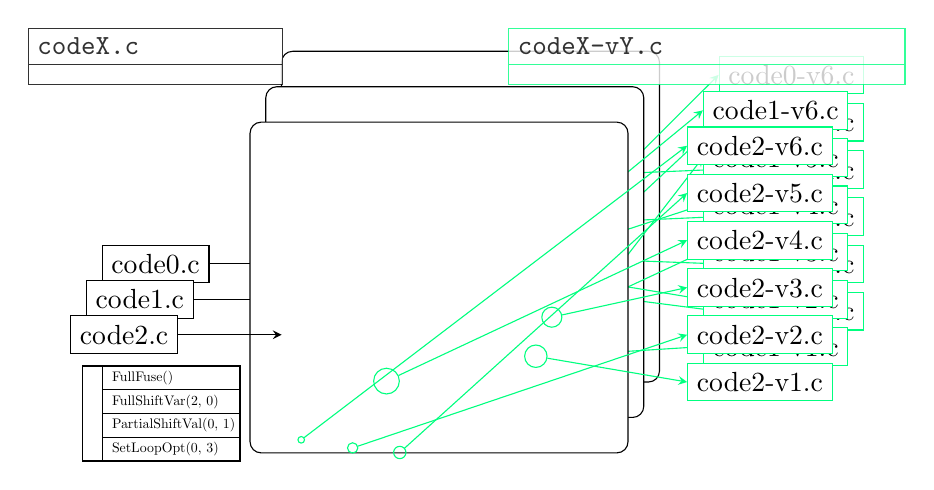
\begin{tikzpicture}
  \foreach \step in {0,1,2}{
    %%% BEGIN main %%%
    \begin{scope}[
      xscale=2, yscale=1.5,
      xshift=-0.1*\step cm, yshift=-0.3*\step cm,
      label/.style={draw=SpringGreen, anchor=east, fill=white}
      ]
      %%% BEGIN cod123.c %%%
      \draw[fill=white, draw, rounded corners] (-1.2, -1.0) rectangle (1.2, 1.8);
      \node[draw, fill=white] at (-2,0) (in-\step) {code\step.c};
      \draw[] (in-\step) edge[-{stealth}] (-1,0);
      %%% END cod123.c %%%
      %%% BEGIN selected %%%
      \foreach [
        evaluate=\i as \xmaru using rand,
        evaluate=\i as \ymaru using rand,
        evaluate=\xmaru \ymaru as \smaru using (1.5-sqrt(\xmaru*\xmaru+\ymaru*\ymaru)),
        evaluate=\i as \time using abs(rand * rand) * 100,
        remember=\xmaru as \lxmaru (initially 0),
        remember=\ymaru as \lymaru (initially 0),
        ] \i in {1,2,...,6}{
        \node[draw, SpringGreen, circle, scale=1*\smaru] at (\xmaru, \ymaru) (ds-\i) {\color{SpringGreen}\CheckmarkBold};
        \node[label] at (2.5, 0.4*\i-0.8) (out-\i) {code\step-v\i.c};
        \draw[SpringGreen] (ds-\i) edge[-{stealth}] (out-\i.west);
      }
      %%% END selected %%%
    \end{scope}
    %%% BEGIN main %%%
  }
  %%% BEGIN many o/x %%%
  \begin{scope}[xscale=2, yscale=1.5, xshift=-0.2cm, yshift=-0.2cm]
    \foreach [
      evaluate=\i as \xmaru using rand,
      evaluate=\i as \xbatsu using rand,
      evaluate=\i as \ymaru using rand,
      evaluate=\i as \ybatsu using rand,
      evaluate=\xmaru \ymaru as \smaru using (1.5-sqrt(\xmaru*\xmaru+\ymaru*\ymaru)),
      evaluate=\xbatsu \ybatsu as \sbatsu using (1.5-sqrt(\xbatsu*\xbatsu+\ybatsu*\ybatsu)),
      remember=\xmaru as \lxmaru (initially 0),
      remember=\ymaru as \lymaru (initially 0),
      ] \i in {1,2,...,40}{
        \node[scale=\sbatsu, opacity=1.2-\sbatsu] at (\xbatsu, \ybatsu) (batsu-\i) {\batsu};
        \node[scale=\smaru, opacity=1.2-\smaru] at (\xmaru, \ymaru) (maru-\i) {\maru};
      }
  %%% BEGIN many o/x %%%
  \end{scope}
  %%% Begin Samples %%%
  \path node [
    scale=0.5,
    draw=black,
    fill=white,
    rectangle split,
    rectangle split parts=4,
    rectangle split part align=left,
  ] at (-3.8cm, -1.9cm)
    (legend) {         \maru{}  FullFuse()
    \nodepart{two}     \maru{}  FullShiftVar(2, 0)
    \nodepart{three}   \maru{}  PartialShiftVal(0, 1)
    \nodepart{four}    \maru{}  SetLoopOpt(0, 3)
  }
  node [anchor=east, SpringGreen] at (legend.west) (leftlegend) {\CheckmarkBold}
  ;
  \node[draw, fit={(leftlegend) (legend)}, inner sep=0] {};
  %%% End Samples %%%
  %%% BEGIN listings %%%
  \path[every node/.style={
    fill=white,
    draw, anchor=north, % clip,
    rectangle split, rectangle split parts=2,
    opacity=0.8,
  }]
  node (inputc)[text width=3cm] at (-4,3) {
    \texttt{codeX.c}\nodepart{two}\usebox\inputc
  } node (outputc)[draw=SpringGreen, text width=4.8cm] at (3,3) {
    \texttt{codeX-vY.c}\nodepart{two}\usebox\outputc
  }
  ;
  %%% BEGIN listings %%%

\end{tikzpicture}
\end{document}
